\vspace{\parskip}
Today we will use {\scshape Desmos} 
to explore the effects of different values of 
\gap{$a$}, \gap{$h$}, \gap{$k$} 
on the graphs of reciprocal functions. 

\begin{tcbraster}[
    raster columns = 2,
    raster equal height,
    raster left skip = 0.5in, raster right skip = 0.5in, raster column skip = 0.75in,
    raster before skip = 0.25in, raster after skip = 0.25in,
]
    \begin{tcolorbox}[]
        \centering
        {\itshape parent function}\\[1\baselineskip]
        \Large
        $ f(x) = \frac{1}{x} $
    \end{tcolorbox}
    \begin{tcolorbox}[]
        \centering
        {\itshape transformed function}\\[1\baselineskip]
        \Large
        $g(x) = \frac{\bm{a}}{(x-\bm{h})} - \bm{k}$
    \end{tcolorbox}
\end{tcbraster}

\vfill 

\begin{myAnnotate}{{Activity}}{To join the {\scshape Desmos} activity\dots}[%
    center,
    width=5.5in,
    before skip = 1\baselineskip,
    colbacktitle=black!15,
    ]
    \begin{itemize}[nosep]
        \item Get out your phone or laptop.
        \item Open a \myEmph{browser} to this URL
        \begin{itemize}
            \item[$\Rightarrow$] {\bfseries\ttfamily https://student.desmos.com/}
        \end{itemize}
        \begin{center}
            \fbox{
\includegraphics[width=4in]{../student-desmos-com.jpg}}
        \end{center}
    \item Continue \myEmph{without} signing in.
        \item Type in your (real!) name.
        \item There are 4 screens in the activity. 
            \begin{center}
                \fbox{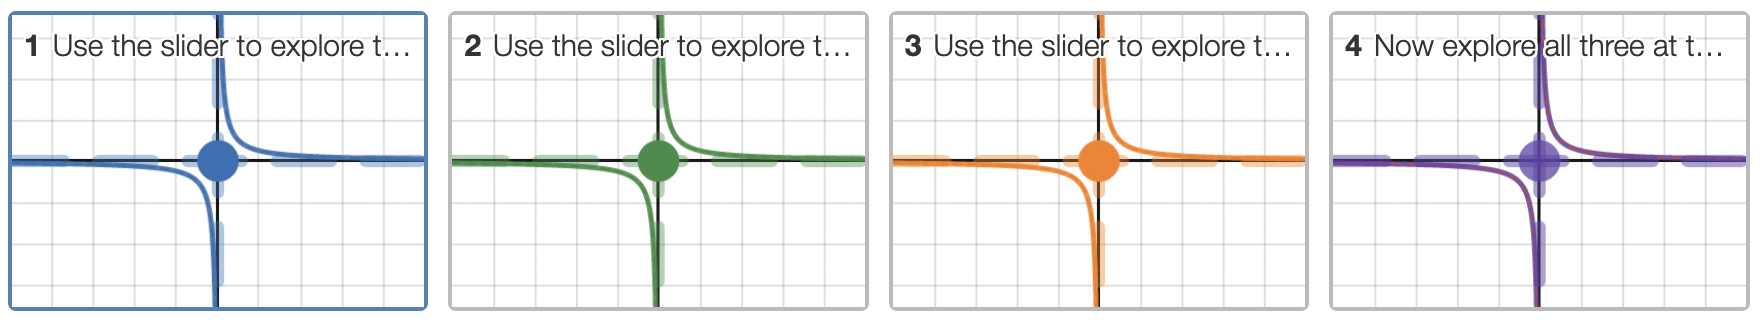
\includegraphics[width=4.5in]{../4-reciprocal-Desmos-screens.png}}
            \end{center}
        \item Go through them \myEmph{one at a time}, 
        and answer the questions on the worksheet.
    \end{itemize}
\end{myAnnotate}

\vfill{}